\newcommand\tab[1][1cm]{\hspace*{#1}}
\graphicspath{{images/}{images/logos/}}
\begin{frame}{Übersicht GUI}
	\begin{center}
		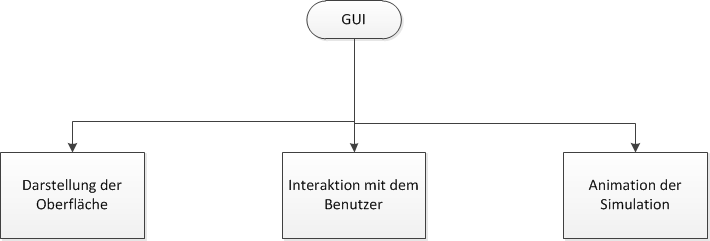
\includegraphics[width=710,height=241]{./model2.png}
	\end{center}
\end{frame}

\begin{frame}{Darstellung der Oberfläche}
	\begin{center}
		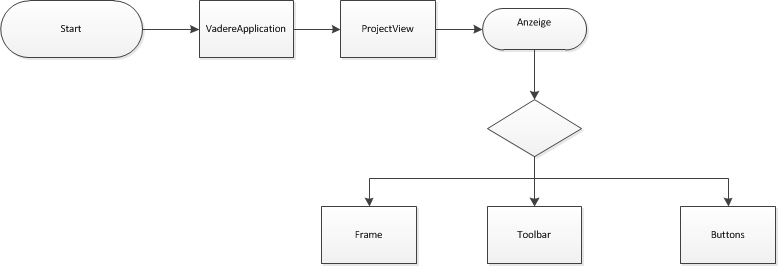
\includegraphics[width=778,height=266]{./model21.png}
	\end{center}
\end{frame}

\begin{frame}{Verwaltung der Actions}
	\begin{center}
		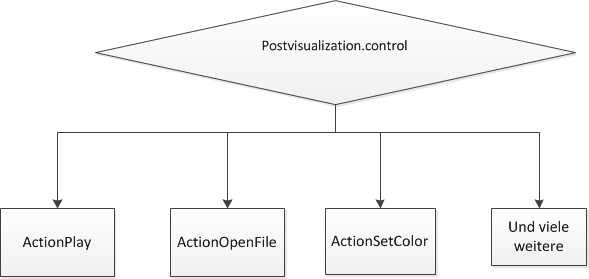
\includegraphics[width=589,height=279]{./model22a.png}
	\end{center}
\end{frame}


\begin{frame}{Verwaltung der Scenarios}
	\begin{center}
		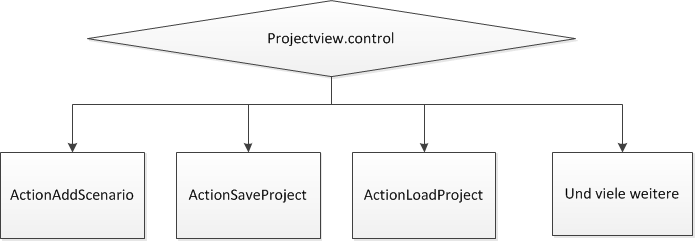
\includegraphics[width=695,height=241]{./model22b.png}
	\end{center}
\end{frame}


\begin{frame}{Zeichnen des Scenarios}
	\begin{center}
		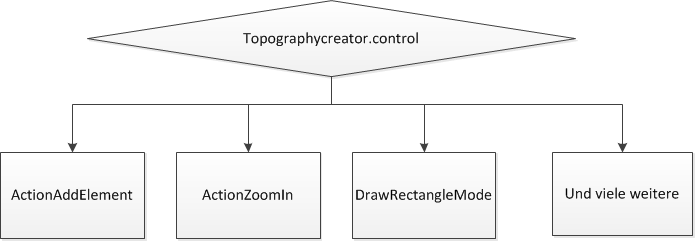
\includegraphics[width=695,height=241]{./model22c.png}
	\end{center}
\end{frame}


\begin{frame}{Animation der Simulation
	\begin{center}
		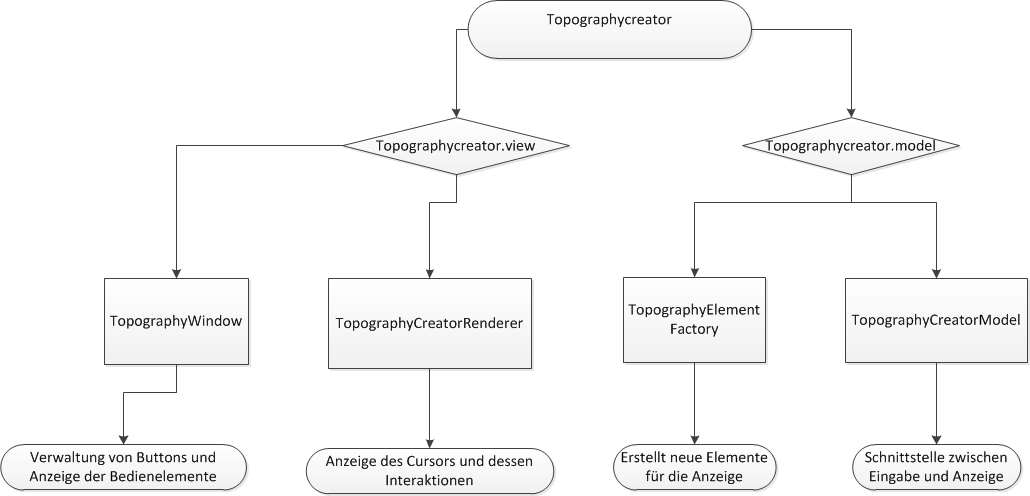
\includegraphics[width=1030,height=496]{./model23a.png}
	\end{center}
\end{frame}

\begin{frame}{Zeichnen der Grafiken}
	\begin{center}
		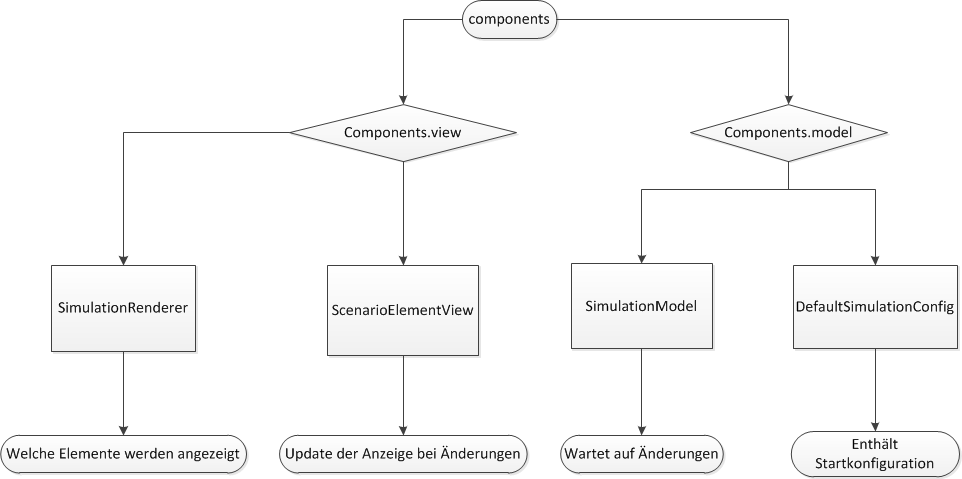
\includegraphics[width=962,height=479]{./model23b.png}
	\end{center}
\end{frame}


\begin{frame}{Button zu Horse}
	\begin{center}
		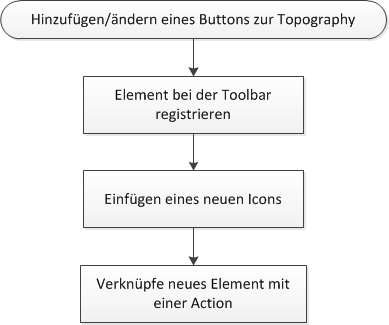
\includegraphics[width=389,height=325]{./model31.png}
	\end{center}
\end{frame}


\begin{frame}{Einbinden der Klasse Horse in GUI}
	\begin{center}
		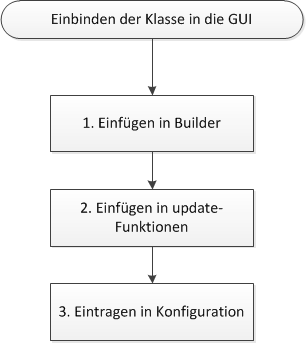
\includegraphics[width=306,height=343]{./model32a.png}
	\end{center}
\end{frame}


\begin{frame}{Einfügen in Builder}
	\begin{center}
		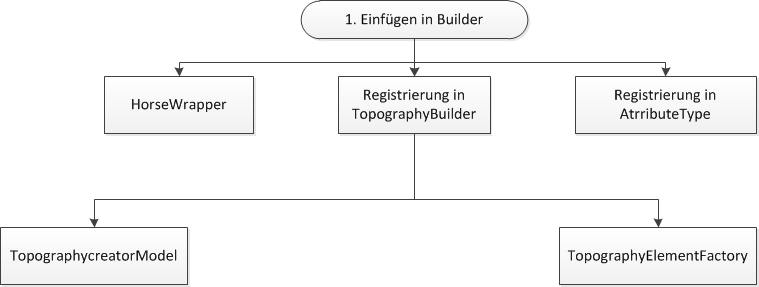
\includegraphics[width=759,height=287]{./model32b.png}
	\end{center}
\end{frame}

\begin{frame}{Einfügen in update - Funktionen}
	\begin{center}
		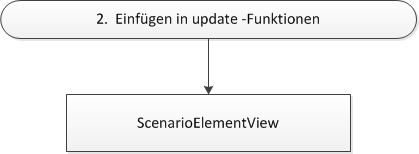
\includegraphics[width=419,height=154]{./model32c.png}
	\end{center}
\end{frame}

\begin{frame}{Eintragen in Konfiguration}
	\begin{center}
		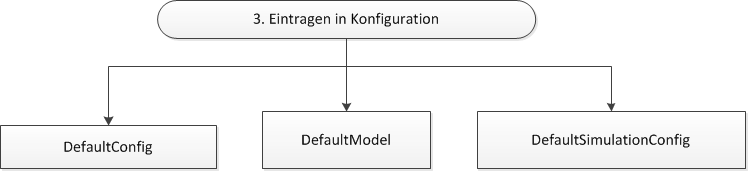
\includegraphics[width=748,height=171]{./model32d.png}
	\end{center}
\end{frame}


